\mysection{The Afterlife}{the-afterlife}

\flavor {
    All our times have come

    Here but now they're gone.

    Seasons don't fear the reaper.

  \Tilde Blue {\UmlautOCap}yster Cult, "Don't Fear The Reaper"
}

Small Gods and Mortals and the beings born of the Dream possess a soul, proof that they are part of reality.  When a Hallowed creature dies it must journey through \mybold{Limbo} to return to the side of \TheAuthority, to be dreamed again. The journey through Limbo takes seven days; souls unable to find their way in time are lost and \mybold{Forgotten}, a dream within the Dream.

Limbo is nowhere and everywhere, a tear in the Dream that separates it from the mind that dreams it. Only the dead can find Limbo; only the dead can hear its call, an incessant whisper beckoning them home. Those who have seen Limbo report that it is a burning metropolis of titanic proportions, ruled by a mad God; others say it is a dead casino-ship orbiting Tartarus; a walled bazaar on the precipice of the Void; an endless necropolis filled with talking ravens.

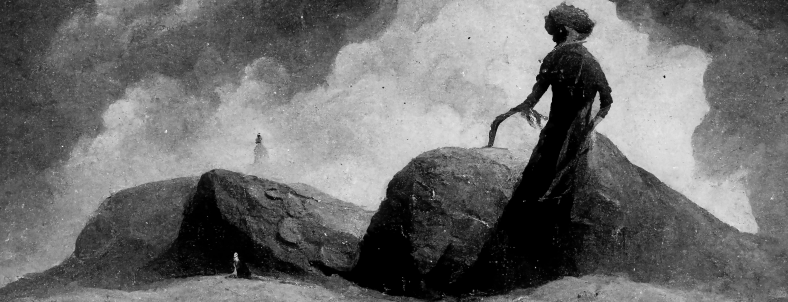
\includegraphics[width=\linewidth,keepaspectratio=true]{totality/AfterlifeHeader}

Seek out the demons and devils that live here and they will gladly barter with you in their shops and dens, where you may trade your soul for favor or protection for living friends and family. Bounty hunters and collectors roam the land searching for those who "bet their souls" in their living days, desperate men and women fleeing their grasp. Gamblers and madmen, the cursed and the damned roll dice in alleys for the greatest prize they'll ever know, the only thing you ever truly have at stake. 

In Limbo, all manner of earthly wonders await. Delights, vices, and temptations abound. Your heart's desire resides in Limbo, and only the most austere can walk through Limbo unmoved or untouched. After seven days, the soul can no longer leave; many have found themselves waiting until the last moment to enjoy the fruits and pleasures of the Dream one last time, and missing the final boat to the far shore.\footnote{The Arbiter is encouraged to make a journey to Limbo into something really epic. Retrieving a soul from the lands of the dead is dangerous to the extreme!}

When an Unseelie dies, they return to the Void, flashing suddenly out of existence as if they never were. Only their closest compatriots will remember their passing, and even then the recollection of their existence quickly fades, like trying to remember a childhood memory or a fading dream. There are no bones of the Unseelie in the graveyards of the Dream.
